\documentclass[11pt,letterpaper,final]{report}
\usepackage[utf8]{inputenc}
\usepackage[francais]{babel}
\usepackage[T1]{fontenc}
\usepackage{amsmath}
\usepackage{amsfonts}
\usepackage{amssymb}
\usepackage{graphicx}
\usepackage{lmodern}
\usepackage[left=2.54cm,right=2.54cm,top=2.54cm,bottom=2.54cm]{geometry}
\begin{document}
\chapter{Modélisation de l'alimentation électronique}
\section{Fonctionnement d'un redresseur monophasé simple alternance}
Le redresseur monophasé simple alternance est composé d'une source de courant alternatif, d'un interrupteur de type IGBT et d'une charge quelquonque tel que présenté à la figure \ref{fig:RedresseurMonophaseSimpleAlternanceIGBT}. Pour les besoin de l'exemple, une charge $RL$ théorique sera utilisée où la résistance se nomme $R$ et l'inductance $L$. De plus, l'on suppose que l'interrupteur IGBT entre en conduction lorsqu'un échelon de tension unitaire est appliqué à la grille de celui-ci. Finalement, en suposant des modèles sans perte, l'équation de circuit se résume à celle présentée à l'équation \ref{eq:RLSimple}. À noter que l'échelon unitaire est défini comme: $u(t<0) = 0, u(t\geq 0) = 1)$.

\begin{figure}[htb!]
	\begin{center}  
		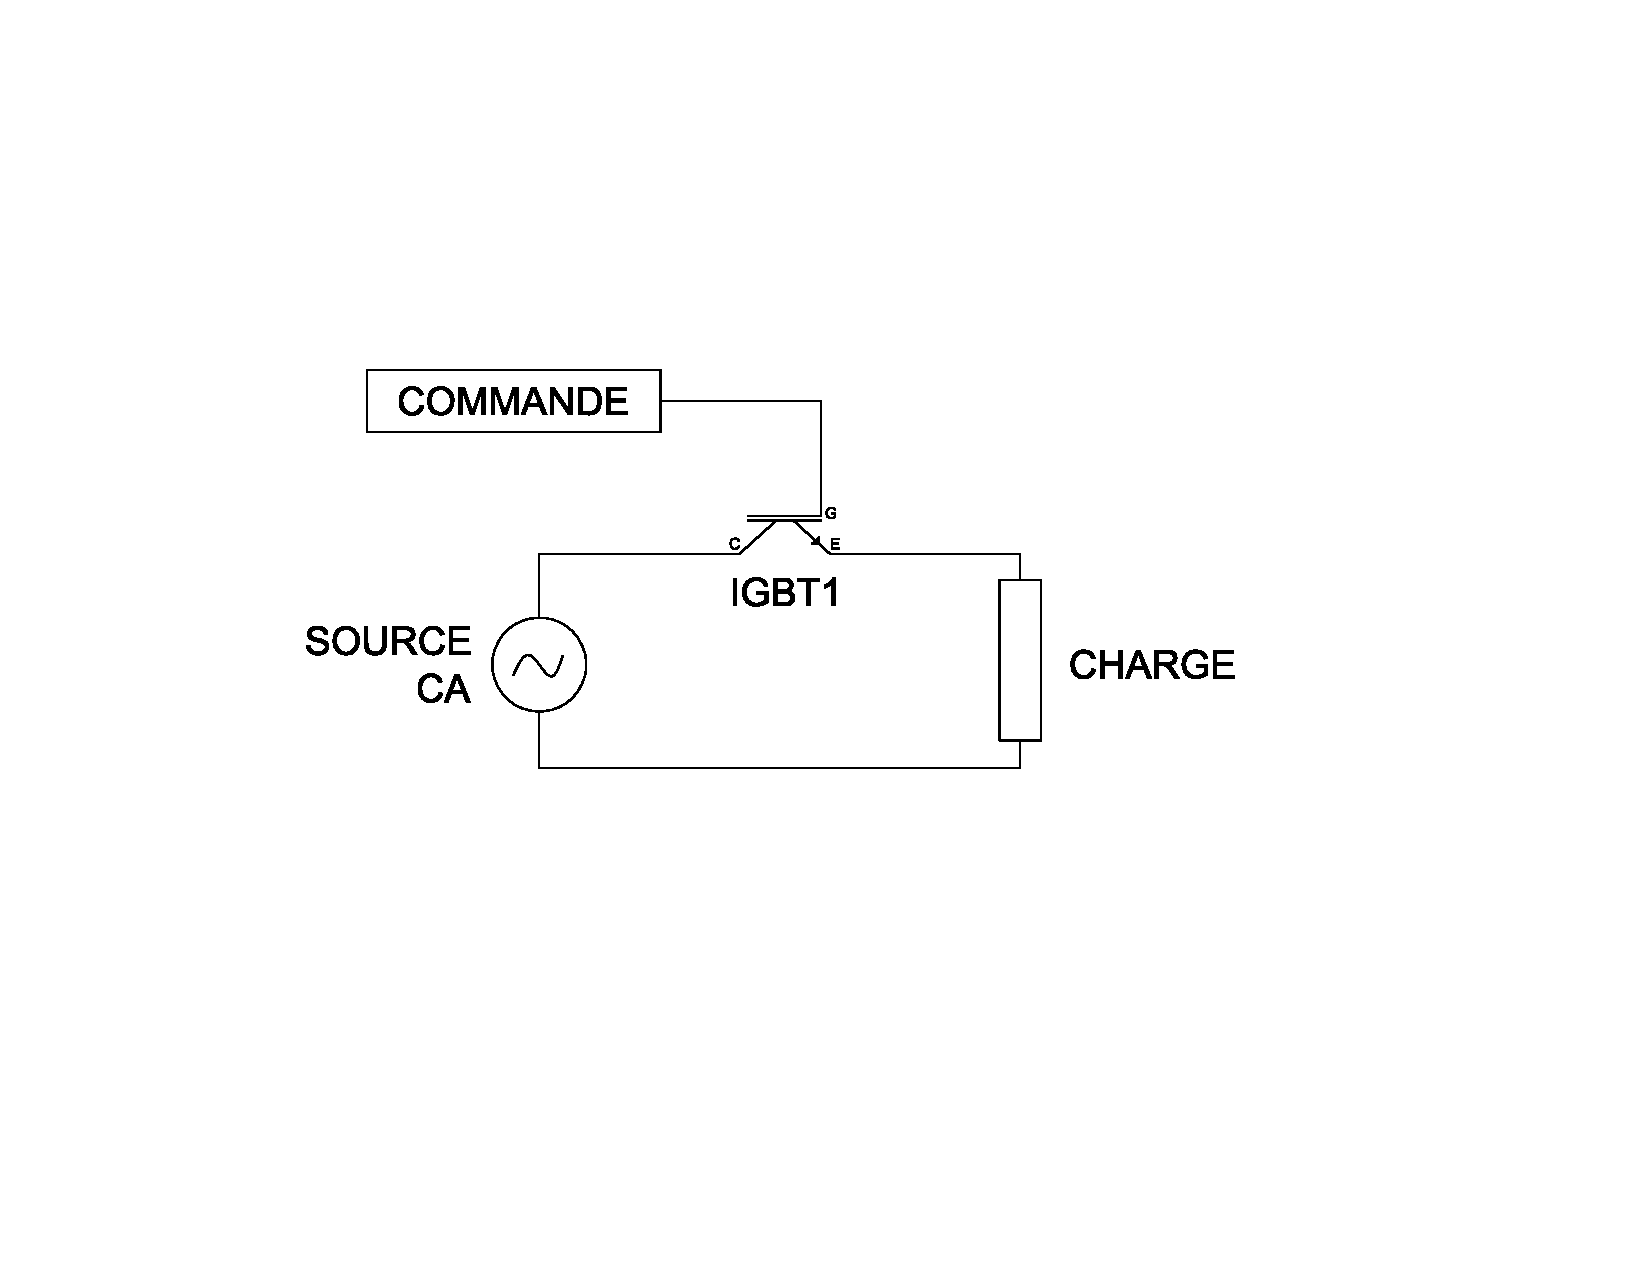
\includegraphics[width=0.7\textwidth]{Circuit/RedresseurMonophaseSimpleAlternanceIGBT}
		\caption{Circuit redresseur monophasé simple alternance avec IGBT et charge quelquonque}
		\label{fig:RedresseurMonophaseSimpleAlternanceIGBT}
	\end{center}   
\end{figure}


\begin{equation}
\label{eq:RLSimple}
v(t) = R i(t) + L \frac{d i(t)}{dt}
\end{equation}

Si l'on néglige la présence de l'IGBT, il est possible d'exprimer le courant dans la charge en fonction de la tension de la source CA:

\begin{eqnarray}
V_{in}(t) &=& E_m\sin{\omega_0 t} \\
|Z| &=& \sqrt{R^2 + (\omega_0 L)^2} \\
\tau &=& \frac{L}{R}\\
\phi &=& \mbox{atan}(\omega_0 \tau) = \mbox{atan}(\omega_0 \frac{L}{R}) \\
\label{eq:solutionRLSimple} i(t) &=& \frac{E_m\sin{\phi}}{|Z|}\mbox{e}^{\frac{-t}{\tau}} + \frac{E_m\sin{(\omega_0 t + \phi})}{|Z|}\\
i(t=0) &=& i_0\\
i(t) &=& i_0  + \frac{E_m\sin{\phi}}{|Z|}\mbox{e}^{\frac{-t}{\tau}} + \frac{E_m\sin{(\omega_0 t + \phi})}{|Z|} \\
\end{eqnarray}

L'équation \ref{eq:solutionRLSimple} est la solution de l'équation différentielle \ref{eq:RLSimple} avec la partie de gauche qui est la composante transitoire et la partie de droite qui est la composante permanente. 

\paragraph{}
Le but principal du redresseur simple alternance est de produire une tension et un courant qui sont strictement positif. Dans le cas du redresseur simple alternance, seulement la partie positive de la source de courant alternative est envoyé à la charge et la partie négative est bloquée par l'IGBT. De plus, gràce à la commande de l'IGBT, il est possible de contrôler le temps de conduction de la partie positive du signal.

Ainsi, si l'on définit le temps total d'une demie période du signal par $T$, le temps de début de conduction de l'IGBT par $t_{on}$ et le temps de début de blocage par $t_{off}$, il est possible de définir le rapport de modulation $m = \frac{t_{off}-t_{on}}{T}$. Supposons un rapport de modulation $m_x$, il est possible, si l'on considère le courant initial nul, d'exprimer le courant dans la charge RL pour une période de modulation étant égale à $T$.

Les figures Ainsi, si l'on choisi le début de conduction ($T_{on}$) à 10\% de la période du signal et une modulation $m_x$ de 0.5, le courant dans la charge RL aura la forme présenté dans la figure

\begin{figure}
        \centering       
        \begin{subfigure}[Séquence directe du réseau à étudier]{
         		\label{fig:RedresseurMonophaseSimpleAlternanceIGBTCourbes50}
                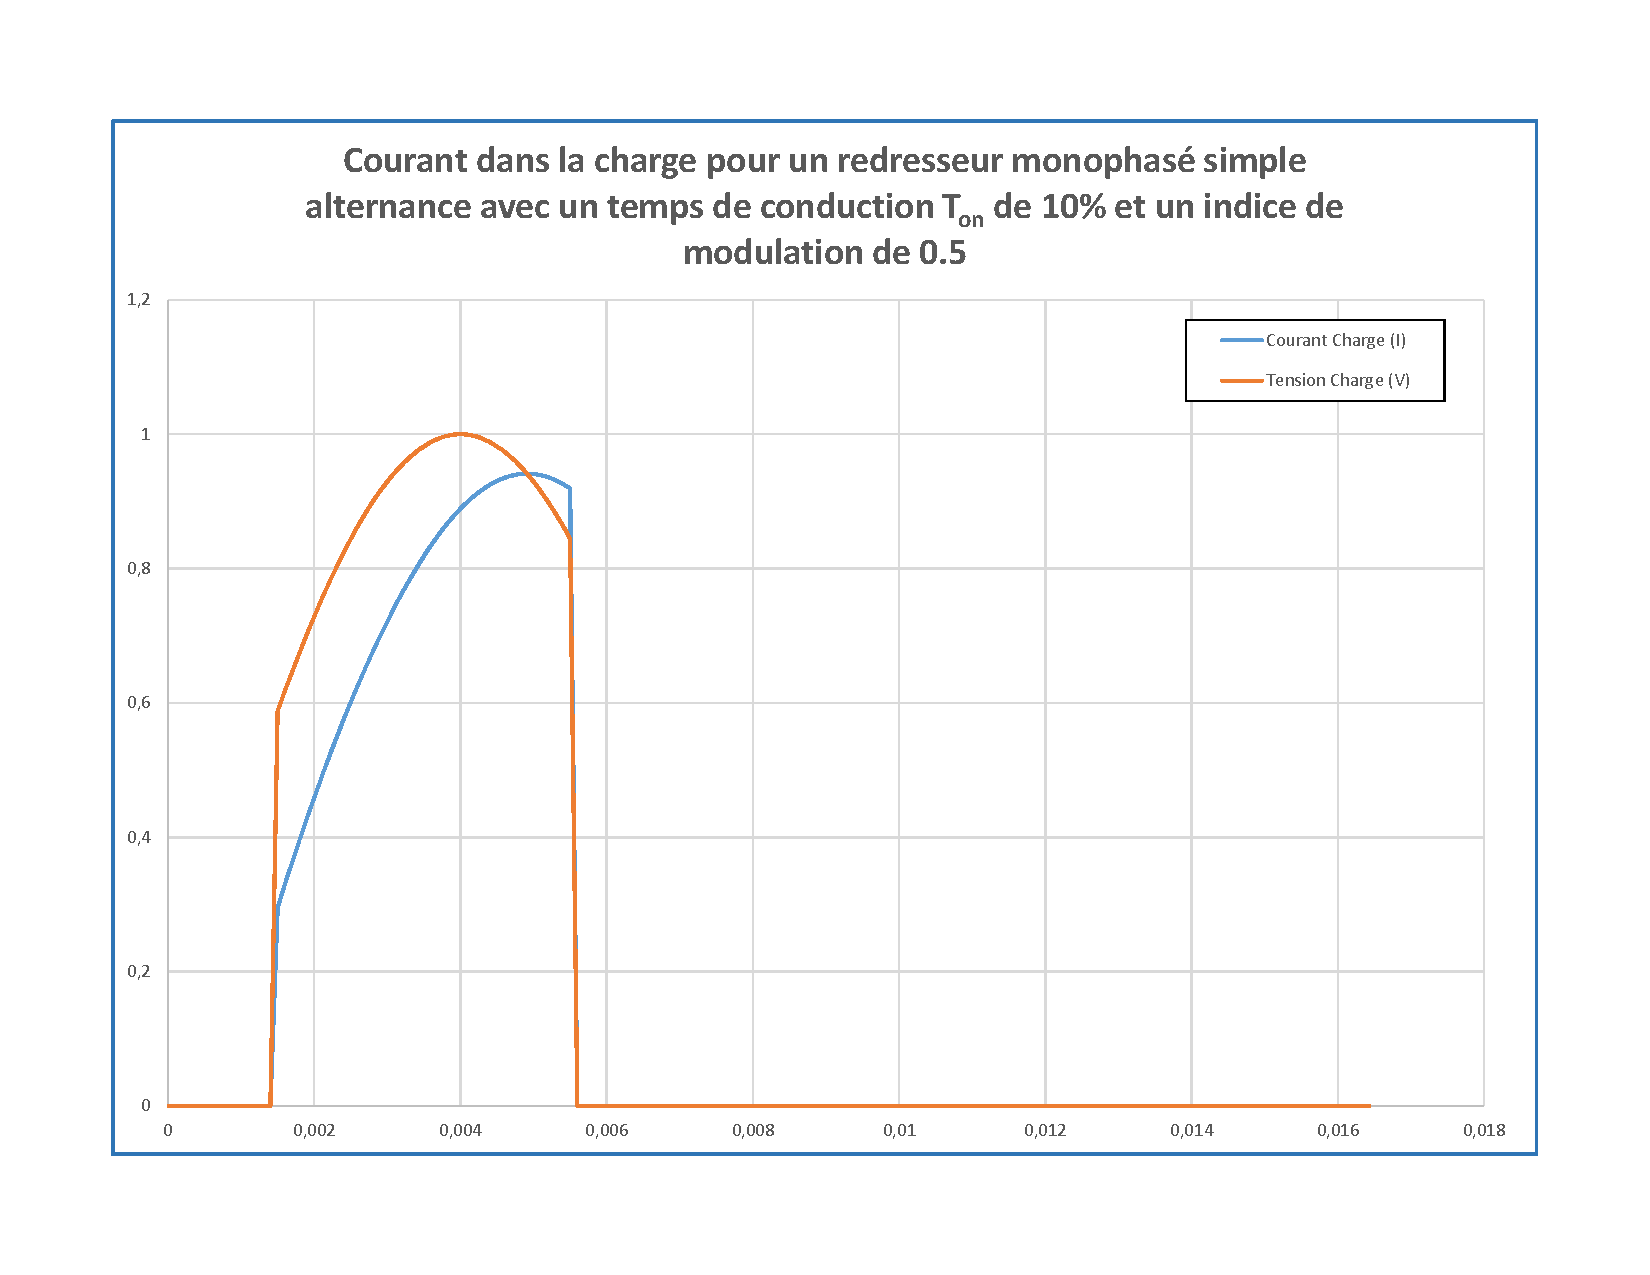
\includegraphics[width=\textwidth]{RedresseurMonophaseSimpleAlternance50}}
        \end{subfigure}
        
        \begin{subfigure}[Séquence inverse du réseau à étudier]{
         		\label{fig:RedresseurMonophaseSimpleAlternanceIGBTCourbes100}
                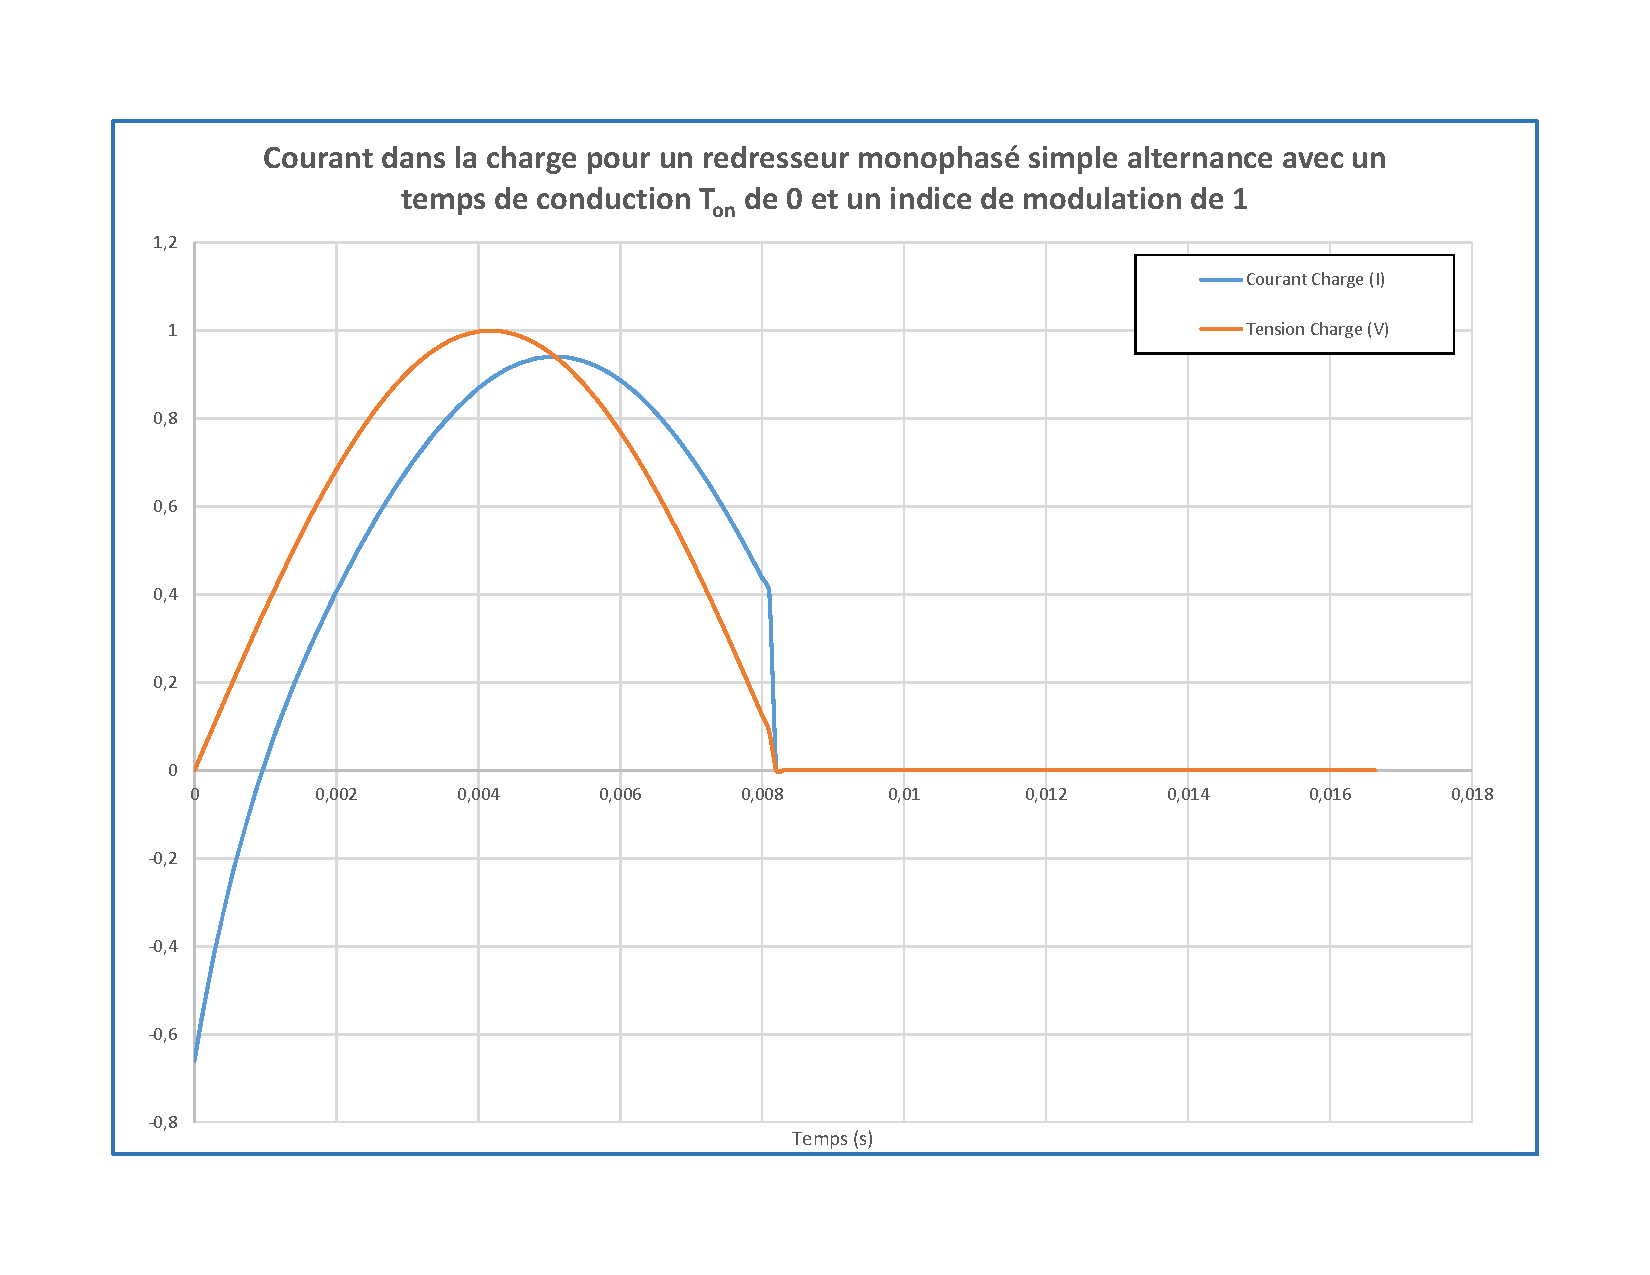
\includegraphics[width=\textwidth]{RedresseurMonophaseSimpleAlternance100}}
        \end{subfigure}
        \caption{Réprésentation des trois séquences du réseau à analyser}\label{fig:RedresseurMonophaseSimpleAlternanceIGBTCourbes}
\end{figure}



Afin de faciliter les calculs, on peut approximer $i(t)$ comme une droite de pente constante. On en déduit que $i(t) = \frac{V_{DC}}{L}t$, pour $0\leq t \leq m_x T$ et $i(t) = \frac{V_{DC}}{L} m_x T \left( 2 - t\right)$, pour $m_x\leq t \leq T$. La valeur moyenne sur une période se calcule comme suit:

\begin{eqnarray}
I_{moy} &=& \int_0^{t_{on}} i(t) + \int_{t_{on}}^{T} i(t)\\
I_{moy} &\approx & \frac{V_{DC}}{LT}\left(\frac{m_x^2 T^2}{2} -(3m_x^2 -4m_x +1)\frac{T^2}{2}\right)
\end{eqnarray}

Par l'analyse des formes d'ondes en traçant le courant moyen en fonction du rapport de modulation, présenté à la figure \ref{eq1}, on remarque que si l'on a un rapport de modulation inférieur à 0.2929, le courant moyen est négatif et que si le rapport de modulation est supérieur à cette valeur, le courant moyen est positif.

\begin{figure}[htb]
\centering
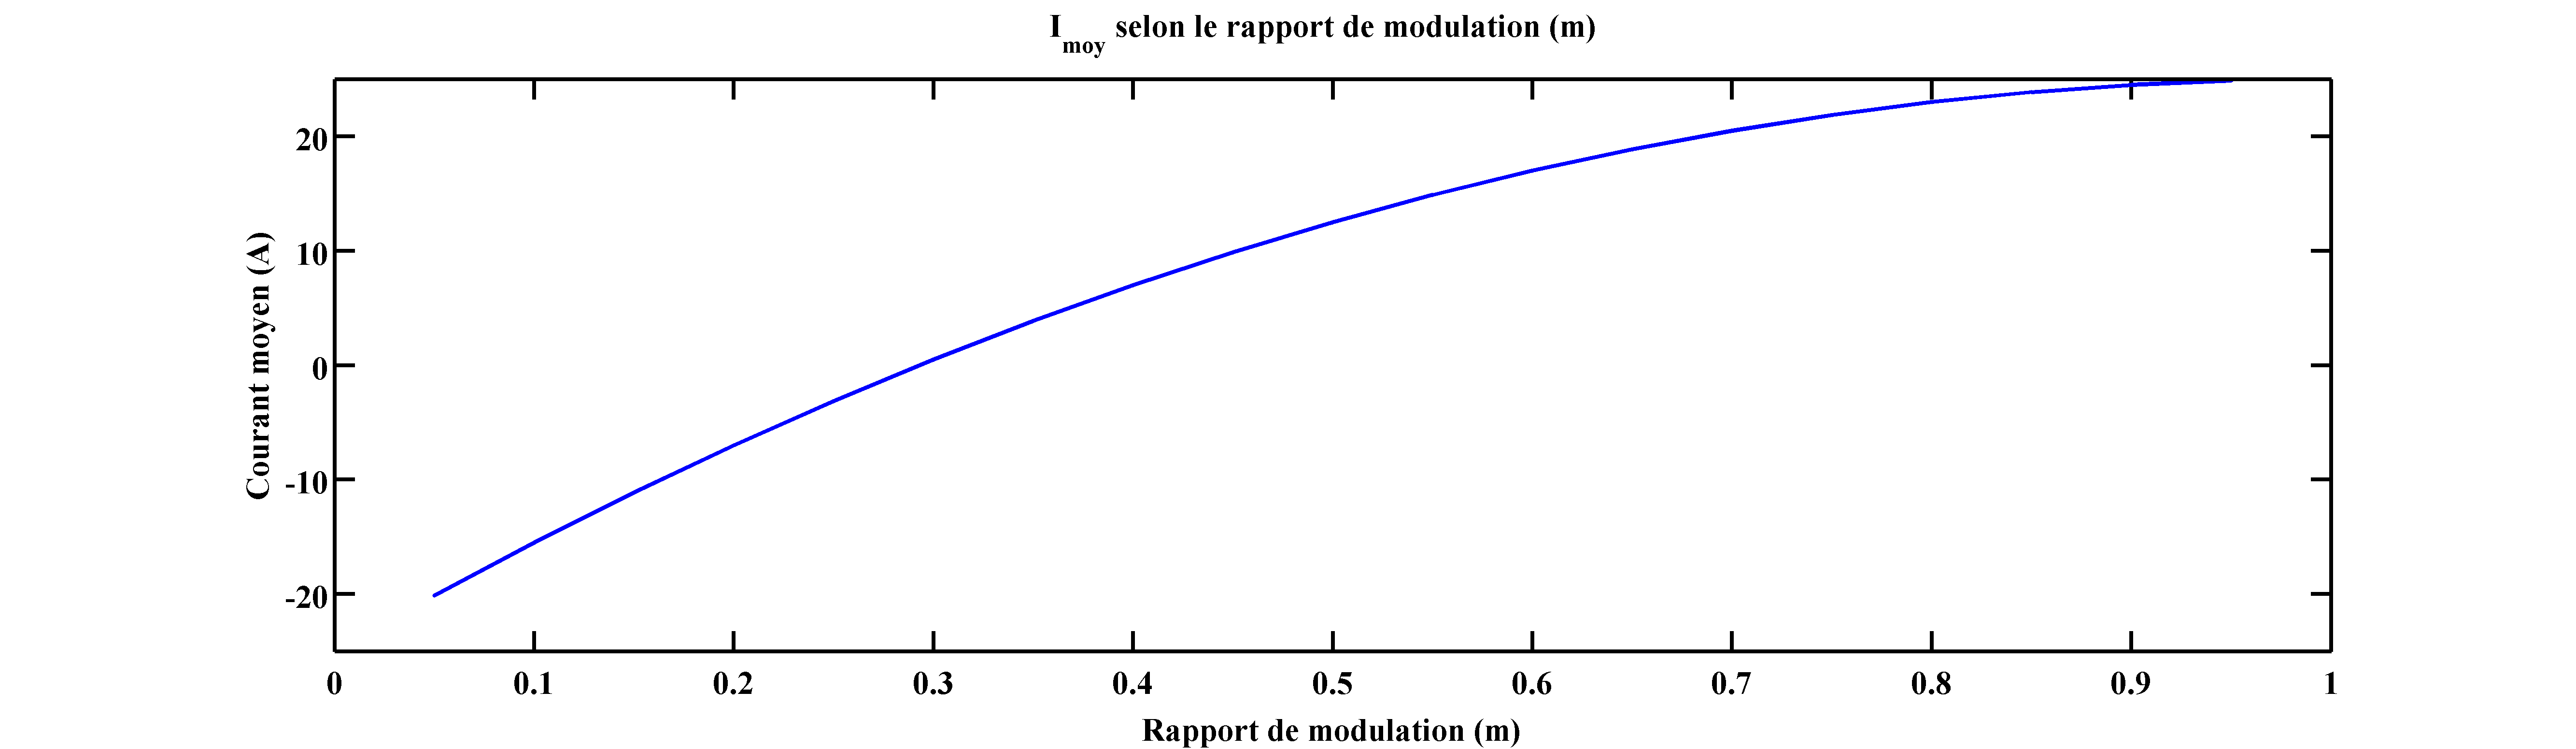
\includegraphics[scale=0.4]{Imoy_m.png}
\caption{Courant moyen en fonction du rapport de modulation dans un onduleur monophasé}
\end{figure}

\section{Fonctionnement d'un onduleur monophasé NPC à 3 niveaux}
Le schéma d'un onduleur monophasé NPC à 3 niveaux est présenté à la figure \ref{eq1}. Un onduleur monophasé NPC à 3 niveaux est composé de 4 transistors, de 6 diodes et de deux condensateurs rattachés au point neutre (point central sur la figure \ref{eq1}). La configuration présentée a pour objectif d'obtenir des niveaux distincts de tension $V_{DC}$ à appliquer aux bornes des électroaimants. Dans cette configuration, chaque transistor ne commute pas toute la tension $V_{DC}$, l'avantage étant qu'on peut utiliser des composantes dont le dimensionnement est moins imposant que celles nécessaire pour fournir une puissance équivalente dans un montage à 2 niveaux classique. 

\paragraph{}Il existe 4 transistors IGBT qui commutent par paires. Les séquences possibles et les tensions produites sont décrites dans le tableau suivant:

\begin{table}[htb]
\centering
\begin{tabular}{ |c|c|c| }
\hline
  Type de séquence & Transistors activés & Niveau de tension \\\hline\hline
  P & [1,2] & $+V_{DC}$ \\\hline
  N & [3,4] & $-V_{DC}$ \\\hline
  O & [1,3] & $0$ \\\hline
  O & [1,4] & $0$ \\\hline
  O & [2,4] & $0$ \\\hline
\end{tabular}
\end{table}

En excluant les états redondants, il existe 3 états distincts, soit l'état P ([1,2]), l'état N([3,4] et l'état 0([1,3]). Une stratégie de commande simple et applicable est celle d'une modulation MLI à plusieurs niveaux. On réfère ici à la figure \ref{fig_MLI_ML} pour une illustration graphique de la commande MLI multiniveaux. À chaque période de commutation, une comparaison entre l'onde désirée et le signal en dent de scie. Pendant la période où le signal est plus grand (en valeur absolue) que le signal en dent de scie, la paire de transistor associée est activée pendant la période de conduction calculée. 
